\documentclass[a4paper]{article}
\usepackage{times}
\usepackage[utf8]{inputenc}
\usepackage[T1]{fontenc}
\usepackage{selinput}
\usepackage{upquote}
\usepackage[margin=2cm, rmargin=4cm, tmargin=3cm]{geometry}
\usepackage{tcolorbox}
\tcbuselibrary{breakable}
\usepackage{xspace}
\usepackage{amsmath}
\usepackage{float}
\usepackage[french]{babel}
\usepackage{hyperref}
\usepackage{xurl}
\usepackage{fontawesome6}
\usepackage{enumitem}
\usepackage{marginnote}
\usepackage{ulem}
\usepackage[yyyymmdd,hhmmss]{datetime}
\usepackage{ulem}
\usepackage{environ}
\usepackage{graphicx}
%\usepackage[top=Bcm, bottom=Hcm, outer=Ccm, inner=Acm, heightrounded, marginparwidth=Ecm, marginparsep=Dcm]{geometry}
\usepackage{courier}



\newtcolorbox{Example}[1]{colback=white,left=20pt,colframe=slideblue,fonttitle=\bfseries,title=#1}
\newtcolorbox{Solutions}[1]{breakable,colback=white,left=20pt,colframe=green,fonttitle=\bfseries,title=#1}
\newtcolorbox{Conseils}[1]{colback=white,left=20pt,colframe=slideblue,fonttitle=\bfseries,title=#1}
\newtcolorbox{Warning}[1]{colback=white,left=20pt,colframe=warning,fonttitle=\bfseries,title=#1}
\newtcolorbox{Note}[1]{colback=white,left=20pt,colframe=grey,fonttitle=\bfseries,title=#1}
\newtcolorbox{Dessin}[1]{colback=white,left=20pt,colframe=grey,fonttitle=\bfseries,title=#1}

\setlength\parindent{0pt}

  %Exercice environment
  \newcounter{exercice}
  \newenvironment{Exercice}[1][]
  {
  \par
  \stepcounter{exercice}\textbf{Question \arabic{exercice}:} (\faClock \enskip \textit{#1})
  }
  {\bigskip}
  

% Title
\newcommand{\titre}{\begin{center}
  \section*{Algorithmes et Pensée Computationnelle}
\end{center}}
\newcommand{\cours}[1]
{\begin{center} 
  \textit{#1}\\
\end{center}
  }



% \newcommand{\exemple}[1]{\newline~\textbf{Exemple :} #1}
\newcommand{\todo}[1]{\textcolor{red}{#1}}
%\newcommand{\attention}[1]{\newline\faExclamationTriangle~\textbf{Attention :} #1}

% Documentation url (escape \# in the TP document)
\newcommand{\documentation}[1]{\faBookOpen~Documentation : \href{#1}{#1}}

% Clef API
\newcommand{\apikey}[1]{\faKey~Clé API : \lstinline{#1}}
\newcommand{\apiendpoint}[1]{\faGlobe~Url de base de l'API \href{#1}{#1}}

%Listing Python style
\usepackage{color}
\definecolor{slideblue}{RGB}{33,131,189}
\definecolor{green}{RGB}{0,190,100}
\definecolor{blue}{RGB}{121,142,213}
\definecolor{grey}{RGB}{120,120,120}
\definecolor{warning}{RGB}{235,186,1}

\usepackage{listings}
\lstdefinelanguage{texte}{
    keywordstyle=\color{black},
    numbers=none,
    frame=none,
    literate=
           {é}{{\'e}}1
           {è}{{\`e}}1
           {ê}{{\^e}}1
           {à}{{\`a}}1
           {â}{{\^a}}1
           {ù}{{\`u}}1
           {ü}{{\"u}}1
           {î}{{\^i}}1
           {ï}{{\"i}}1
           {ë}{{\"e}}1
           {Ç}{{\,C}}1
           {ç}{{\,c}}1
           {ô}{{\^o}}1,
    columns=fullflexible,keepspaces,
	breaklines=true,
	breakatwhitespace=true,
}
\lstset{
  language=Python,
	%basicstyle=\bfseries\footnotesize,
  basicstyle=\footnotesize\ttfamily\small,
	breaklines=true,
	breakatwhitespace=true,
	commentstyle=\color{grey},
	stringstyle=\color{slideblue},
  keywordstyle=\color{slideblue},
	morekeywords={with, as, True, False, Fraction, Float, join, index, None, main, argparse, self, sort, __eq__, __add__, __mul__ ,__ne__, __radd__, __del__, __ge__, __gt__, split, os, endswith, is_file, scandir, @classmethod, this},
	deletekeywords={id},
	showspaces=false,
	showstringspaces=false,
	columns=fullflexible,keepspaces,
	literate=
           {é}{{\'e}}1
           {è}{{\`e}}1
           {ê}{{\^e}}1
           {à}{{\`a}}1
           {â}{{\^a}}1
           {ù}{{\`u}}1
           {ü}{{\"u}}1
           {î}{{\^i}}1
           {ï}{{\"i}}1
           {ë}{{\"e}}1
           {Ç}{{\,C}}1
           {ç}{{\,c}}1
           {ô}{{\^o}}1,
    numbers=left,
}

\newtcbox{\mybox}{nobeforeafter,colframe=white,colback=slideblue,boxrule=0.5pt,arc=1.5pt, boxsep=0pt,left=2pt,right=2pt,top=2pt,bottom=2pt,tcbox raise base}
\newcommand{\projet}{\mybox{\textcolor{white}{\small projet}}\xspace}
\newcommand{\optionnel}{\mybox{\textcolor{white}{\small Optionnel}}\xspace}
\newcommand{\advanced}{\mybox{\textcolor{white}{\small Pour aller plus loin}}\xspace}
\newcommand{\auto}{\mybox{\textcolor{white}{\small Auto-évaluation}}\xspace}


\usepackage{environ}
\newif\ifShowSolution
\NewEnviron{solution}{
  \ifShowSolution
	\begin{Solutions}{\faTerminal \enskip Solution}
		\BODY
	\end{Solutions}
  \fi}

\usepackage{environ}
\newif\ifShowExample
\NewEnviron{exemple}{
  \ifShowExample
	\begin{Example}{\faTerminal \enskip Exemple}
		\BODY
	\end{Example}
  \fi}

\usepackage{environ}
 \newif\ifShowConseil
  \NewEnviron{conseil}{
    \ifShowConseil
    \begin{Conseils}{\faLightbulb \quad Conseil}
      \BODY
    \end{Conseils}

    \fi}

    \usepackage{environ}
  \newif\ifShowWarning
  \NewEnviron{attention}{
    \ifShowWarning
    \begin{Warning}{\faTriangleExclamation \quad Attention}
      \BODY
    \end{Warning}

    \fi}

  \newif\ifShowNote
  \NewEnviron{note}[1]{
    \ifShowNote
    \begin{Note}{\faEye \quad Comment added by #1 at \date - \currenttime}
      \BODY
    \end{Note}

    \fi}  

    \newif\ifShowDessin
    \NewEnviron{dessin}[1]{
      \ifShowDessin
      \begin{Dessin}{\faPen \quad Figure}
        \BODY
      \end{Dessin}
  
      \fi}  

%\newcommand{\Conseil}[1]{\ifShowIndice\ \newline\faLightbulb[regular]~#1\fi}

\usepackage[T1]{fontenc}
\usepackage{float}
\setlist[itemize]{label=\textbullet}


\begin{document}

% Change the following values to true to show the solutions or/and the hints
\ShowSolutiontrue
\ShowConseiltrue
\titre
\cours{Algorithmes de tri et Complexité - exercices basiques}

Le but de cette série d'exercices est d'aborder les notions présentées durant la séance de cours. Cette série d'exercices sera orientée autour des points suivants:
\begin{enumerate}
    \item La récursivité
    \item La complexité des algorithmes
    \item Les algorithmes de tri
\end{enumerate}

Les exercices de cette séance seront réalisés en Java et Python. \\

Le temps indiqué (\faClock) est à titre indicatif.

\section{Récursivité}

Le but principal de la récursivité est de résoudre un gros problème en le divisant en plusieurs petites parties à résoudre. \\

\begin{Exercice}[10 minutes] \textbf{Somme des chiffres} \\
    Écrivez une fonction récursive en Python et en Java qui prend un entier en paramètre et retourne la somme des chiffres dont il est composé. Par exemple, la somme des chiffres de 126 est: 1+2+6 = 9.
    
    \begin{conseil}
    Pour obtenir le chiffre des unités d'un nombre, utilisez l'opérateur modulo \texttt{\%}. Par exemple: $42 \bmod 10 = 2$, car le reste de la division entière de 42 par 10 est 2.
    Ensuite, pour obtenir le chiffre 4, effectuez une division entière par 10 : en Python, \texttt{42 // 10} vaut 4, en Java, \texttt{42 / 10} vaut 4, car les deux opérandes sont des entiers.
    \end{conseil}
    
    \begin{solution}
    \textbf{Python :}
        \lstinputlisting{solutions/SumDigits.py}
                
    \textbf{Java :}
       \lstinputlisting{solutions/SumDigits.java}
    
    \end{solution}
\end{Exercice}

\section{Complexité}

 \begin{figure}[H]
        \centering
        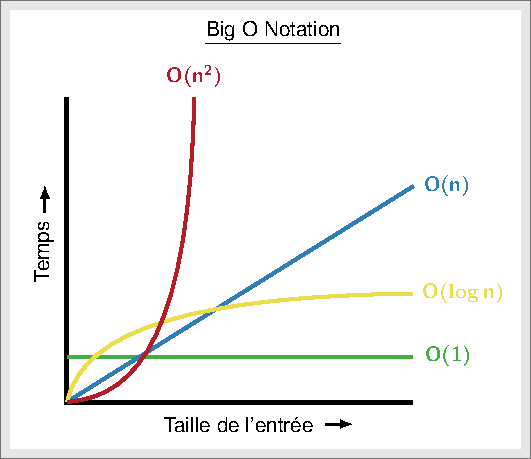
\includegraphics[width=9cm]{images/complexity.pdf}
        \caption{Représentation de complexités temporelles. La complexité décrit la façon dont le temps d'exécution \textbf{croît asymptotiquement} lorsque la taille des données augmente, et non sa valeur exacte.}
        \label{bigO}
\end{figure}

Indiquez en une phrase, ce que font ces algorithmes ci-dessous et calculez leur complexité temporelle avec la notation $O$. Le code est écrit en Python et en Java. \\

\begin{Exercice}[10 minutes] \textbf{Complexité} \\

    Quelle est la complexité des programmes ci-dessous?\\
    \textbf{Python:}
    \begin{lstlisting}{language=Python}
# Entrée: n un nombre entier
def algo(n):
    s = 0
    for i in range(10*n):
        s += i
    return s \end{lstlisting}
    
    \textbf{Java:}
    \begin{lstlisting}{language=Java}
public static int algo(int n) {
    int s = 0;
    for (int i=0; i < 10*n; i++){
        s += i;
    }
    return s;
}  \end{lstlisting}

    \begin{enumerate}[label=(\Alph*)]
        \item $O(n)$
        \item $O(n^3)$
        \item $O(\log(n))$
        \item $O(n^n)$
    \end{enumerate}
    
    \begin{conseil}
    Rappelez-vous que la notation $O$ sert à exprimer la complexité d'algorithmes dans le \textbf{pire des cas}. Les règles suivantes vous seront utiles. Soit $n$ la taille de vos données. On a alors:
    \begin{enumerate}
        \item Les constantes sont ignorées : $O(2n) = 2 \cdot O(n) = O(n)$
        \item Les termes dominés sont ignorés : $O(2n^2+5n+50)$ = $O(n^2)$
    \end{enumerate}
    \end{conseil}

    \begin{solution}
        L'algorithme est composé d'une boucle qui incrémente une variable \lstinline{s}. Il effectue l'opération d'addition $10 \cdot n$ fois et par conséquent a une complexité de $O(n)$ comme les facteurs constants sont ignorés.
    \end{solution}
\end{Exercice}


\begin{Exercice}[10 minutes] \textbf{Complexité} \\
    Soit \lstinline|values| une liste de longueur $n$. Quelle est la complexité des programmes ci-dessous?\\
    \textbf{Python :}
    \begin{lstlisting}[language=Python]
# Entrée: values est une liste de nombres entiers et threshold un nombre entier
def algo(values, threshold):
    i = 0
    while i < len(values) and values[i] <= threshold:
        i += 1
    s = i - 1
    return s
    \end{lstlisting}
    
    \textbf{Java :}
    \begin{lstlisting}[language=Java]
public static int algo(int[] values, int threshold) {
    int i = 0;
    while (i < values.length && values[i] <= threshold){
        i += 1;
    }
    int s = i - 1;
    return s;
}
    \end{lstlisting}

    \begin{enumerate}[label=(\Alph*)]
        \item $O(n^3)$
        \item $O(\log(n))$
        \item $O(n)$
        \item $O(n^n)$
    \end{enumerate}

    \begin{solution}
    L'algorithme est composé d'une boucle \lstinline{while} qui parcourt la liste \texttt{values} jusqu'à trouver une valeur supérieure à \texttt{threshold}. Ainsi, dans le pire des cas, l'algorithme parcourt toute la liste, et a donc une complexité de $O(n)$, où $n$ est la taille de la liste.
    \end{solution}
\end{Exercice}
\begin{Exercice}[10 minutes] \textbf{Complexité} \\
    Quelle est la complexité des programmes ci-dessous?\\
        \textbf{Python :}
        \begin{lstlisting}[language=Python]
# Entrée: first_values et second_values sont deux listes de nombres entiers
def algo(first_values, second_values):
    n = len(first_values)
    m = len(second_values)
    for i in range(n):
        first_values[i] = first_values[i]*2
    for j in range(m):
        second_values[j] = second_values[j]%2
        \end{lstlisting}
        
        \textbf{Java :}
        \begin{lstlisting}[language=Java]
public static void algo(int[] firstValues, int[] secondValues) {
    int n = firstValues.length;
    int m = secondValues.length;
    for (int i=0; i < n; i++){
        firstValues[i] = firstValues[i]*2;
    }
    for (int j=0; j < m; j++){
        secondValues[j] = secondValues[j]%2;
    }
}
        \end{lstlisting}

        \begin{enumerate}[label=(\Alph*)]
            \item $O(n^2)$
            \item $O(n + m)$
            \item $O(n)$
            \item $O(2^n)$
        \end{enumerate}

        \begin{solution}
        L'algorithme est composé de deux boucles. La première parcourt la liste \texttt{first\_values} en Python (\texttt{firstValues} en Java) et multiplie par 2 ses éléments.
        L'autre parcourt la liste \texttt{second\_values} en Python (\texttt{secondValues} en Java) et affecte à chaque élément le reste de la division euclidienne de l'élément par 2.
        Soient $n$ et $m$ les tailles respectives de ces deux listes, on obtient une complexité de $O(n + m)$.
        Comme les boucles sont exécutées l'une après l'autre, leurs complexités s'additionnent.
        \end{solution}
\end{Exercice}

\begin{Exercice}[10 minutes] \textbf{Complexité} \\
    Quelle est la complexité des programmes ci-dessous?\\
    \textbf{Python :}
    \begin{lstlisting}[language=Python]
# Entrée: values est une liste de nombres entiers
import math
def algo(values):
    n = len(values)
    i = 1
    s = 0
    while i < n:
        s += values[i]
        i = 2*i
    return s
    \end{lstlisting}
    
    \textbf{Java:}
    \begin{lstlisting}[language=Java]
import java.lang.Math; 

public static int algo(int[] values) {
    int n = values.length;
    int i = 1;
    int s = 0;
    while (i < n){
        s += values[i];
        i = 2*i;
    }
    return s;
} \end{lstlisting}

    \begin{enumerate}[label=(\Alph*)]
        \item $O(n^2)$
        \item $O(n)$
        \item $O(\log(n))$
        \item $O(n^n)$
    \end{enumerate}

    \begin{solution}
    L'algorithme consiste en une boucle qui ajoute à la variable $s$ les valeurs de la liste \texttt{values}, à condition que les indices de ces valeurs soient des puissances de 2 inférieures à $n$. La variable \texttt{i} prend successivement les valeurs $1, 2, 4, \ldots, 2^{\lfloor \log_2(n) \rfloor}$. \\ 

    Pour montrer que $2^{\lfloor \log_2(n) \rfloor}$ est la plus grande puissance de 2 inférieure ou égale à $n$, remarquons que $n = 2^{\log_2(n)}$ et que $2^{\lfloor \log_2(n) \rfloor} \leq n < 2^{\lfloor \log_2(n) \rfloor + 1}$. Ainsi, $n$ est encadré par deux puissances de 2 consécutives. \\
    
    En réécrivant la suite des valeurs de \texttt{i} sous la forme $2^0, 2^1, \ldots, 2^{\lfloor \log_2(n) \rfloor}$, on constate que la boucle effectue $\lfloor \log_2(n) \rfloor$ itérations, d'où une complexité en $O(\lfloor \log_2(n) \rfloor) = O(\log(n))$, puisque la notation $O$ décrit une croissance asymptotique et non des valeurs exactes.
    \end{solution}    

\end{Exercice}

\begin{Exercice}[10 minutes] \textbf{Complexité \optionnel} \\
    Quelle est la complexité du programme ci-dessous?\\
        \textbf{Python :}
        \begin{lstlisting}[language=Python]
# Entrée: n un nombre entier
def algo(n):
    m = 0
    for i in range(n):
        for j in range(i):
            m += i+j
    return m
        \end{lstlisting}
        
        \textbf{Java :}
        \begin{lstlisting}[language=Java]
public static int algo(int n) {
    int m = 0;
    for (int i=0; i < n; i++){
        for (int j=0; j < i; j++){
            m += i+j;
        }
    }
    return m;
}
        \end{lstlisting}
    
        \begin{enumerate}[label=(\Alph*)]
            \item $O(n^2)$
            \item $O(n)$
            \item $O(\log(n))$
            \item $O(2^n)$
        \end{enumerate}

    \begin{solution} 
    L'algorithme est composé de deux boucles imbriquées.
    La boucle extérieure est exécutée $n$ fois.
    Le nombre d'itérations de la boucle intérieure dépend de l'itération courante de la boucle extérieure : pour une valeur donnée de \texttt{i}, la boucle intérieure est exécutée \texttt{i} fois. Comme \texttt{i} prend successivement les valeurs $0, 1, \ldots, n-1$, le nombre total d'exécutions de l'instruction \lstinline{m += i+j} est:
    \[
        0 + 1 + 2 + \cdots + (n-1)
        = \sum_{i=0}^{n-1} i
        = \frac{n(n-1)}{2}
        = \frac{n^2}{2} - \frac{n}{2}.
    \]
    Chaque exécution de cette instruction prend un temps constant. On ne conserve que le terme quadratique, car il définit le comportement asymptotique de la fonction: les termes dominés et les facteurs constants sont ignorés. La complexité temporelle est donc $O(n^2)$.
    \end{solution}
    
\end{Exercice}

\section{Algorithmes de Tri}

\begin{Exercice}[15 minutes] [Python] \textbf{Insertion dans une liste triée}\\
    Soit un nombre entier \lstinline{n}, et une liste triée \lstinline{l}. Ecrivez un programme Python qui insère la valeur \lstinline{n} dans la liste \lstinline{l} tout en s'assurant que la liste \lstinline{l} reste triée.

    \lstinputlisting{code/IntInsertion.py}

    \begin{Example}{\faTerminal \quad Exemple}
        En passant les arguments suivants à votre programme: \texttt{n=5} et \texttt{l=[2,4,6]}. Ce dernier devra retourner \lstinline{l =[2,4,5,6]}
    \end{Example}

    \begin{solution}
        \lstinputlisting{solutions/IntInsertion.py}
    \end{solution}


\end{Exercice}

\begin{Exercice} [30 minutes] [Python] \textbf{Tri fusion (Merge Sort)} \\
    Étant donné deux listes triées, on peut construire une liste triée contenant tous leurs éléments (leur \textit{fusion}). Elle repose sur l'observation que si les deux listes sont triées, le plus petit élément de la liste fusionnée est soit le premier élément de la première liste, soit le premier élément de la seconde. On construit donc la liste finale élément par élément: à chaque étape, on compare les premiers éléments des deux listes, on retire le plus petit et on l'ajoute à la fin de liste finale. Dès que l'une des deux listes est vide, il suffit d'ajouter à la suite les éléments restants de l'autre. \\
    
    Les étapes à suivre pour implémenter l'algorithme sont les suivantes:
    \begin{enumerate}
        \item Si la lsite n'a qu'un seul élément, il est déjà trié.
        \item Sinon, séparer la liste en deux parties plus ou moins égales.
        \item Trier récursivement les deux parties avec l'algorithme de tri fusion.
        \item Fusionner les deux listes triées dans une seule liste triée.
    \end{enumerate}
    
    Soit la liste \lstinline{l} suivante [38, 27, 43, 3, 9, 82, 10], triez les éléments de la liste en utilisant un tri fusion. Combien d'itération effectuez-vous?
    
    \begin{itemize}
        \item \textbf{Python :}
            \lstinputlisting{code/MergeSort.py}
    \end{itemize}
    
    \begin{conseil}
    \begin{itemize}
        \item L'algorithme est récursif. 
        \item Revenez à la visualisation de l'algorithme dans les diapositives 81 à 109 pour comprendre comment fonctionne concrètement le tri fusion. 
    \end{itemize}
    
    \end{conseil}

    \begin{conseil}
\textbf{Théorème 1} \quad La récurrence
\begin{align*}
T(n) &= a\,T(n/b) + c n^{k} \\
T(1) &= c
\end{align*}

où $a$, $b$, $c$ et $k$ sont des constantes, se résout comme suit :

\begin{align*}
T(n) &\in O(n^{k}) \quad \text{si } a < b^{k} \\
T(n) &\in O(n^{k} \log n) \quad \text{si } a = b^{k} \\
T(n) &\in O(n^{\log_{b}{a}}) \quad \text{si } a > b^{k}
\end{align*}

    \end{conseil}
    
    \begin{solution}
        \textbf{Python :}
        \lstinputlisting[language=python, lastline=30]{solutions/MergeSort.py}
    \end{solution}

    \begin{solution}
\lstinputlisting[language=python, firstline=31, firstnumber=31]{solutions/MergeSort.py}
    \end{solution}
   
    \begin{solution}
        Le tri fusion est un algorithme récursif. Ainsi, nous pouvons exprimer sa complexité temporelle via une relation de récurrence : $T(n) = 2T(n/2) + O(n)$. En effet, l'algorithme comporte 3 étapes :
        \begin{enumerate}
            \item ``Divide Step'', qui divise les listes en deux sous-listes, et cela prend un temps constant
            \item ``Conquer Step'', qui trie récursivement les sous-listes de taille $n/2$ chacune, et cette étape est représentée par le terme $2T(n/2)$ dans l'équation.
            \item La dernière étape consiste à fusionner les listes, sa complexité est de $O(n)$.
        \end{enumerate}
        La solution à cette équation est $O(n \log n)$.
    \end{solution}
\end{Exercice}


\begin{Exercice} [20 minutes] [Python] \textbf{Tri à bulles (Bubble Sort)} \\
    Le tri à bulles consiste à parcourir plusieurs fois une liste en comparant les éléments deux à deux, côte à côte. Pour trier la liste par ordre croissant, on échange les deux éléments si celui de gauche est plus grand que celui de droite. Sinon, on les laisse à leur place.\\

    Après chaque comparaison, on avance d'une position dans la liste. À la fin du premier passage, le plus grand élément se trouve donc à la fin de la liste, à sa position définitive. On recommence sur la partie de la liste qui n'est pas encore triée, jusqu'à ce qu'un passage complet ne provoque aucun échange: la liste est alors triée.
    
    \begin{itemize}
            \item \textbf{Python :}
                \lstinputlisting{code/BubbleSort.py} 
        \end{itemize}
       
        \ \\
        
        \begin{solution}
        \textbf{Python :}
        \lstinputlisting{solutions/BubbleSort.py}
    \end{solution}
    \begin{solution}
        À chaque passage de la boucle extérieure, le plus grand élément de la partie encore non triée est placé à sa position définitive. La boucle intérieure effectue donc une comparaison de moins au passage suivant : le nombre total de comparaisons est
        \[
            (n-1) + (n-2) + \cdots + 1 + 0 = \frac{n(n-1)}{2}.
        \]
        Chaque comparaison et chaque échange prennent un temps constant. Le terme dominant étant quadratique, la complexité temporelle est $O(n^2)$. Dans cette implémentation, tous les passages sont effectués même si la liste est déjà triée, car aucun arrêt anticipé n'est prévu.
    \end{solution}
    
    \end{Exercice}

\end{document}
